\documentclass[12pt]{article}%
\usepackage{amsfonts}
\usepackage{fancyhdr}
\usepackage{comment}
\usepackage[a4paper, top=2.5cm, bottom=2.5cm, left=2.2cm, right=2.2cm]%
{geometry}
\usepackage{times}
\usepackage{amsmath}
\usepackage{changepage}
\usepackage{amssymb}
\usepackage{graphicx}%
\setcounter{MaxMatrixCols}{30}
%\usepackage{hyperref}


%These tell TeX which packages to use.
\usepackage{array,epsfig}
\usepackage{amsmath}
\usepackage{amsfonts}
\usepackage{amssymb}
\usepackage{amsxtra}
\usepackage{amsthm}
\usepackage{mathrsfs}
\usepackage{color}





\usepackage{listings}
\usepackage{longtable}
\definecolor{codegreen}{rgb}{0,0.6,0}
\definecolor{codegray}{rgb}{0.5,0.5,0.5}
\definecolor{codepurple}{rgb}{0.58,0,0.82}
\definecolor{backcolour}{rgb}{0.96,0.96,0.94}
\lstdefinestyle{mystyle}{
	backgroundcolor=\color{backcolour},
	commentstyle=\color{codegreen},
	keywordstyle=\color{blue},
	numberstyle=\tiny\color{codegray},
	stringstyle=\color{codepurple},
	basicstyle=\footnotesize,
	breakatwhitespace=false,
	breaklines=true,
	captionpos=b,
	keepspaces=true,
	numbers=left,
	numbersep=5pt,
	showspaces=false,
	showstringspaces=false,
	showtabs=false,
	tabsize=2
}
\lstset{style=mystyle}

















%%%%%%%%% hyperref %%%%%%%%%%%%
\usepackage[pdftex,letterpaper=true,pdfpagelabels=true,pagebackref=true,bookmarks]{hyperref} 
% with basic options
% pagebackref=true provides links back from the References to the body text. This can cause trouble for printing.

%%%%%%%% cref cleverref %%%%%%%%%%%

% cref package must be loaded after hyperref !
\usepackage[noabbrev]{cleveref}




%Here I define some theorem styles and shortcut commands for symbols I use often
\theoremstyle{definition}
\newtheorem{defn}{Definition}
\newtheorem{thm}{Theorem}
\newtheorem*{thm*}{Theorem}
\newtheorem{cor}{Corollary}
\newtheorem*{rmk}{Remark}
\newtheorem{lem}{Lemma}
\newtheorem*{joke}{Joke}
\newtheorem{ex}{Example}
\newtheorem*{soln}{Solution}
\newtheorem{prop}{Proposition}




\newtheorem{sol}{Solution}


\newtheorem{theorem}{Theorem}
\newtheorem{acknowledgement}[theorem]{Acknowledgement}
\newtheorem{algorithm}[theorem]{Algorithm}
\newtheorem{axiom}{Axiom}
\newtheorem{case}[theorem]{Case}
\newtheorem{claim}[theorem]{Claim}
\newtheorem{conclusion}[theorem]{Conclusion}
\newtheorem{condition}[theorem]{Condition}
\newtheorem{conjecture}[theorem]{Conjecture}
\newtheorem{corollary}[theorem]{Corollary}
\newtheorem{criterion}[theorem]{Criterion}
\newtheorem{definition}[theorem]{Definition}
\newtheorem{example}[theorem]{Example}
\newtheorem{exercise}[theorem]{Exercise}
\newtheorem{lemma}[theorem]{Lemma}
\newtheorem{notation}[theorem]{Notation}
\newtheorem{problem}[theorem]{Problem}
\newtheorem{proposition}[theorem]{Proposition}
\newtheorem{remark}[theorem]{Remark}
\newtheorem{solution}[theorem]{Solution}
\newtheorem{summary}[theorem]{Summary}
%\newenvironment{proof}[1][Proof]{\textbf{#1.} }{\ \rule{0.5em}{0.5em}}

\newcommand{\Q}{\mathbb{Q}}
\newcommand{\R}{\mathbb{R}}
\newcommand{\C}{\mathbb{C}}
\newcommand{\Z}{\mathbb{Z}}


% operators
\DeclareMathOperator{\rank}{{rank}}
\DeclareMathOperator{\argmin}{{argmin}}
\DeclareMathOperator{\argmax}{{argmax}}
\DeclareMathOperator{\flatt}{{flat}}
\DeclareMathOperator{\sym}{{sym}}
\DeclareMathOperator{\sgn}{sgn}
\DeclareMathOperator{\conv}{conv}
\DeclareMathOperator{\env}{env}
\DeclareMathOperator{\dist}{dist}
\DeclareMathOperator{\epi}{epi}
\DeclareMathOperator{\Id}{Id}
\DeclareMathOperator{\dom}{dom}
\DeclareMathOperator{\cl}{cl}
\DeclareMathOperator{\Normal}{Normal}


% matrices
\newcommand{\bbm}{\begin{bmatrix}}
\newcommand{\ebm}{\end{bmatrix}}
\newcommand{\bem}{\begin{pmatrix}}
\newcommand{\eem}{\end{pmatrix}}

% parentheses
%\newcommand{\l[}{\left[}
%\newcommand{\r]}{\right]}
%\newcommand{\l(}{\left(}
%\newcommand{\r)}{\right)}

% 
\def\<{\langle}
\def\>{\rangle}

\usepackage{cite}



%%%%%%%%%%%% Mathcal{ } %%%%%%%
%%%%%%%%%%%%%%%%%%%%%%%%%%%%%%%
\newcommand{\cA}{{\mathcal A}}
\newcommand{\cB}{{\mathcal B}}
\newcommand{\cC}{{\mathcal C}}
\newcommand{\cD}{{\mathcal D}}
\newcommand{\cE}{{\mathcal E}}
\newcommand{\cF}{{\mathcal F}}
\newcommand{\cG}{{\mathcal G}}
\newcommand{\cDQ}{{\mathcal {DQ}}}
\newcommand{\cH}{{\mathcal H}}
\newcommand{\cI}{{\mathcal I}}
\newcommand{\cJ}{{\mathcal J}}
\newcommand{\cK}{{\mathcal K}}
\newcommand{\cL}{{\mathcal L}}
\newcommand{\cM}{{\mathcal M}}
\newcommand{\cN}{{\mathcal N}}
\newcommand{\cO}{{\mathcal O}}
\newcommand{\cP}{{\mathcal P}}
\newcommand{\cQ}{{\mathcal Q}}
\newcommand{\cR}{{\mathcal R}}
\newcommand{\cS}{{\mathcal S}}
\newcommand{\cT}{{\mathcal T}}
\newcommand{\cDP}{{\mathcal {DP}}}
\newcommand{\cU}{{\mathcal U}}
\newcommand{\cV}{{\mathcal V}}
\newcommand{\cW}{{\mathcal W}}
\newcommand{\cX}{{\mathcal X}}
\newcommand{\cY}{{\mathcal Y}}
\newcommand{\cZ}{{\mathcal Z}}

%%%%%%%%%%%% Mathbb{ } %%%%%%%%
%%%%%%%%%%%%%%%%%%%%%%%%%%%%%%%
\newcommand{\bA}{{\mathbb A}}
\newcommand{\bB}{{\mathbb B}}
\newcommand{\bC}{{\mathbb C}}
\newcommand{\bD}{{\mathbb D}}
\newcommand{\bE}{{\mathbb E}}
\newcommand{\bF}{{\mathbb F}}
\newcommand{\bG}{{\mathbb G}}
\newcommand{\bH}{{\mathbb H}}
\newcommand{\bI}{{\mathbb I}}
\newcommand{\bJ}{{\mathbb J}}
\newcommand{\bK}{{\mathbb K}}
\newcommand{\bL}{{\mathbb L}}
\newcommand{\bM}{{\mathbb M}}
\newcommand{\bN}{{\mathbb N}}
\newcommand{\bO}{{\mathbb O}}
\newcommand{\bP}{{\mathbb P}}
\newcommand{\bQ}{{\mathbb Q}}
\newcommand{\bR}{{\mathbb R}}
\newcommand{\bS}{{\mathbb S}}
\newcommand{\bT}{{\mathbb T}}
\newcommand{\bU}{{\mathbb U}}
\newcommand{\bV}{{\mathbb V}}
\newcommand{\bW}{{\mathbb W}}
\newcommand{\bX}{{\mathbb X}}
\newcommand{\bY}{{\mathbb Y}}
\newcommand{\bZ}{{\mathbb Z}}



\begin{document}
	
	\title{CPSC 532W Homework 6}
	\author{Naomi Graham}
	\date{\today}
	\maketitle
	
	All the code can be found on: \url{https://github.com/n6graham/cpsc532_hw6}.
	


	
	%\begin{figure}[h]
	
%	I printed the terminal output from running the unit tests to give incontrovertible proof that they all passed.
%	\newline
%		\includegraphics[scale=0.6]{foppl}
%		\includegraphics[scale=0.6]{hoppl}
%		\includegraphics[scale=0.6]{prob}
%	\end{figure}
	
	
%	\newpage
	
	
	\section{Program 1}
	
	\begin{center}
		 \begin{tabular}{||c || c c c ||} 
		 \hline
		\multicolumn{4}{|c|}{Program 1} \\
		 \hline
		 Number of particles & Z (evidence) & Mean & Variance \\ [0.5ex] 
		 \hline\hline
		 1 & 1 & 3 & nan  \\ 
		 \hline
		 10 & 1 & 99.1000 & 7639.2109  \\
		 \hline
		 100 & 1 & 80.4600 & 8960.1699  \\
		 \hline
		 1000 & 1 & 101.5100 & 10413.6953  \\  
		 \hline
		 10 000 & 1 & 99.5248 & 9983.4941  \\ [1ex]
		 \hline
		 100 000 & 1 & 99.4249 & 10061.4521  \\ [1ex]
		 \hline
		\end{tabular}
	\end{center}
	
	\begin{figure}[h]
	\centering
	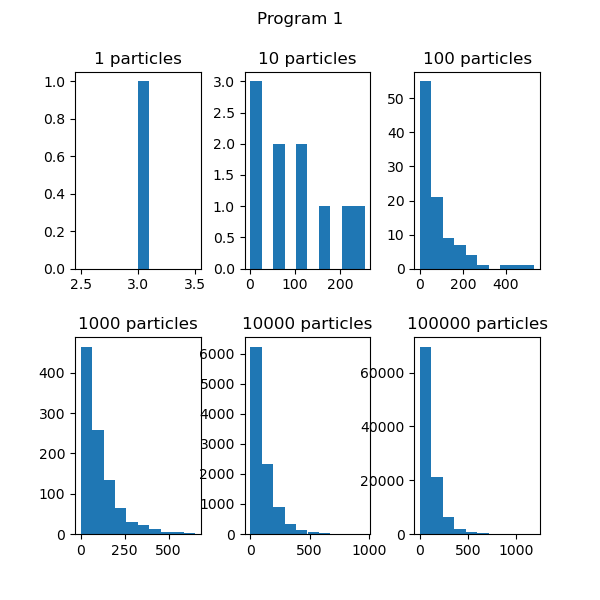
\includegraphics[scale=0.6]{program1_hist}
	\end{figure}
		
		
		\newpage
		
		
		\section{Program 2}
	
	
		\begin{center}
			 \begin{tabular}{||c || c c c ||} 
			 \hline
			\multicolumn{4}{|c|}{Program 2} \\
			 \hline
			 Number of particles & Z (evidence) & Mean & Variance \\ [0.5ex] 
			 \hline\hline
			 1 & 3.5531e-10 & 2.3191 & nan  \\ 
			 \hline
			 10 & 0.0016 & 6.8162 & 2.5264e-13  \\
			 \hline
			 100 & 0.0007 & 8.7266 & 0.3422 \\
			 \hline
			 1000 & 0.0002 & 6.8198 & 0.4003  \\  
			 \hline
			 10 000 & 0.0002 & 7.2663 & 0.9606  \\ [1ex]
			 \hline
			 100 000 & 0.0003 & 7.2832 & 0.8407  \\ [1ex]
			 \hline
			\end{tabular}
		\end{center}
		
		
		\begin{figure}[h]
		\centering
		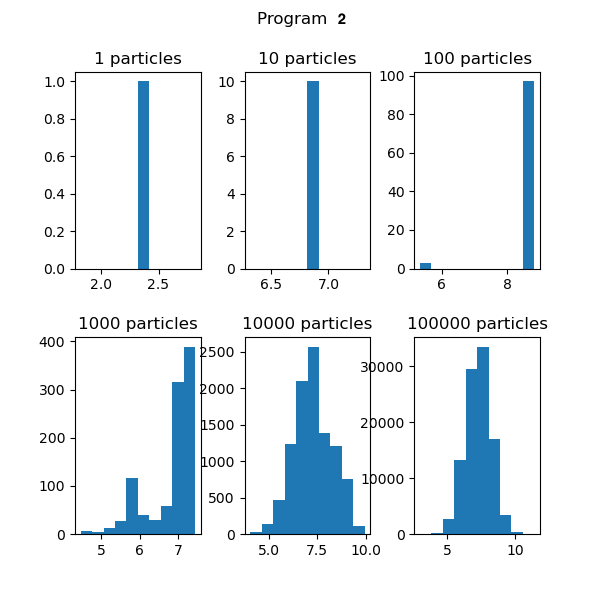
\includegraphics[scale=0.8]{program2_hist}
		\end{figure}
			
			
			\newpage
			
			
			\section{Program 3}
	
	\begin{center}
				 \begin{tabular}{||c || c c c ||} 
				 \hline
				\multicolumn{4}{|c|}{Program 3} \\
				 \hline
				 N & Z  & Mean & Variance \\ [0.5ex] 
				 \hline\hline
				 1 & 5.54e-23 & 
				 $\begin{pmatrix}
				1.0 & 2.0 & 1.0 & 1.0 & 2.0 \\ 1.0 & 0.0 & 2.0 & 2.0 & 2.0 \\ 2.0 & 0.0 & 2.0 & 2.0 & 2.0 \\ 2.0 & 0.0& & &
				 \end{pmatrix}$ 
				 & $\begin{pmatrix}  
				0.0 & 0.0 & 0.0 & 0.0 & 0.0 \\ 0.0 & 0.0 & 0.0 & 0.0 & 0.0 \\ 0.0 & 0.0 & 0.0 & 0.0 & 0.0 \\ 0.0 & 0.0 & & &
				 \end{pmatrix} $ \\ 
				 \hline
				 10 & 5.11e-20 & 
				 $\begin{pmatrix} 
				 0.6 & 1.3 & 1.0 & 1.7 & 1.0 \\ 2.0 & 2.0 & 2.0 & 1.0 & 0.0 \\ 0.0 & 2.0 & 2.0 & 2.0 & 2.0 \\ 2.0 & 1.0& & &
				 \end{pmatrix} $ & 
				 $\begin{pmatrix}
				 0.8 & 0.6 & 0.6 & 0.2 & 0.0 \\ 0.0 & 0.0 & 0.0 & 0.0 & 0.0 \\ 0.0 & 0.0 & 0.0 & 0.0 & 0.0 \\ 0.0 & 0.0 & & &
				 \end{pmatrix} $  \\
				 \hline
				 100 & 3.26e-20 & 
				 $\begin{pmatrix}
				 1.6 & 1.6 & 1.9 & 1.8 & 1.0 \\ 1.3 & 1.6 & 1.7 & 1.8 & 1.6 \\ 0.5 & 1.6 & 1.6 & 1.7 & 1.8 \\ 1.6 & 0.6& & &
				  \end{pmatrix} $ & 
				 $\begin{pmatrix}  
				 0.6 & 0.6 & 0.2 & 0.3 & 0.0 \\ 0.8 & 0.5 & 0.5 & 0.1 & 0.7 \\ 0.8 & 0.2 & 0.2 & 0.2 & 0.2 \\ 0.2 & 0.5 & & & 
				 \end{pmatrix} $  \\
				 \hline
				 1000 & 5.98e-20 & 
				 $\begin{pmatrix} 
				 1.5 & 1.6 & 1.7 & 1.7 & 1.0 \\ 1.5 & 1.8 & 1.8 & 1.7 & 1.1 \\ 0.1 & 1.6 & 1.7 & 1.8 & 1.9 \\ 1.5 & 1.0& & &
				  \end{pmatrix} $ & 
				 $\begin{pmatrix}  
				 0.7 & 0.6 & 0.4 & 0.4 & 0.0 \\ 0.6 & 0.3 & 0.2 & 0.3 & 1.0 \\ 0.2 & 0.5 & 0.4 & 0.2 & 0.1 \\ 0.4 & 0.7 & & &
				 \end{pmatrix} $  \\  
				 \hline
				 10 000 & 5.98e-20 & 
				 $\begin{pmatrix} 
				  1.5 & 1.6 & 1.7 & 1.7 & 1.0 \\ 1.5 & 1.8 & 1.8 & 1.7 & 1.1 \\ 0.1 & 1.6 & 1.7 & 1.8 & 1.9 \\ 1.5 & 1.0& & &
				  \end{pmatrix} $ & 
				 $\begin{pmatrix}  
				 0.7 & 0.6 & 0.4 & 0.4 & 0.0 \\ 0.6 & 0.3 & 0.2 & 0.3 & 1.0 \\ 0.2 & 0.5 & 0.4 & 0.2 & 0.1 \\ 0.4 & 0.7 & & & 
				 \end{pmatrix} $  \\ [1ex]
				 \hline
				 100 000 & & 
				 $\begin{pmatrix}  \end{pmatrix} $ & 
				 $\begin{pmatrix}  \end{pmatrix} $  \\ [1ex]
				 \hline
				\end{tabular}
		\end{center}

	

	

	
	\begin{figure}[h]
	\section{Program 3}
	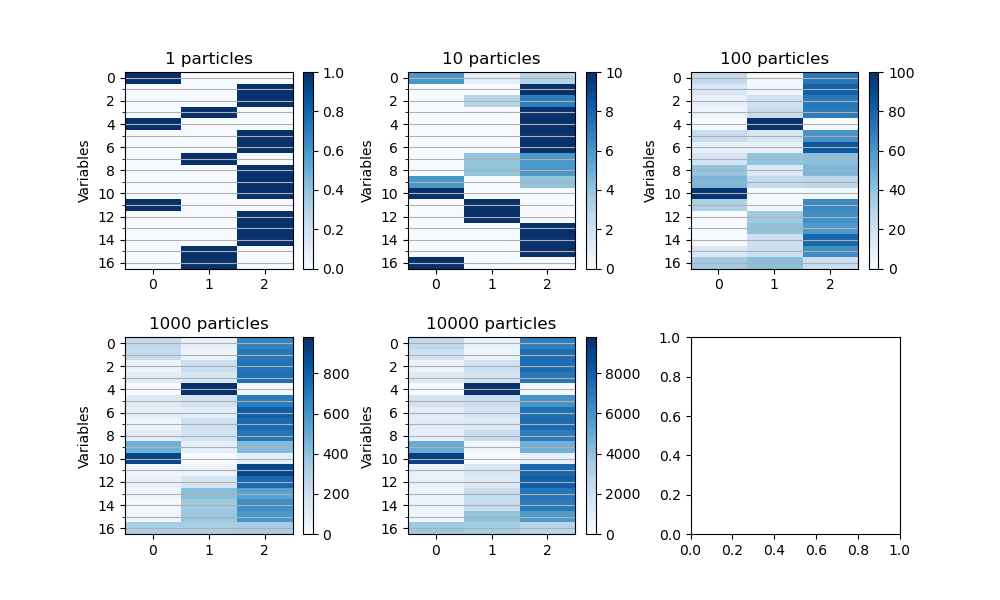
\includegraphics[scale=0.75]{program3_hist}
	\end{figure}
	
%	\begin{figure}[h]
%	\section{Program 4}
%		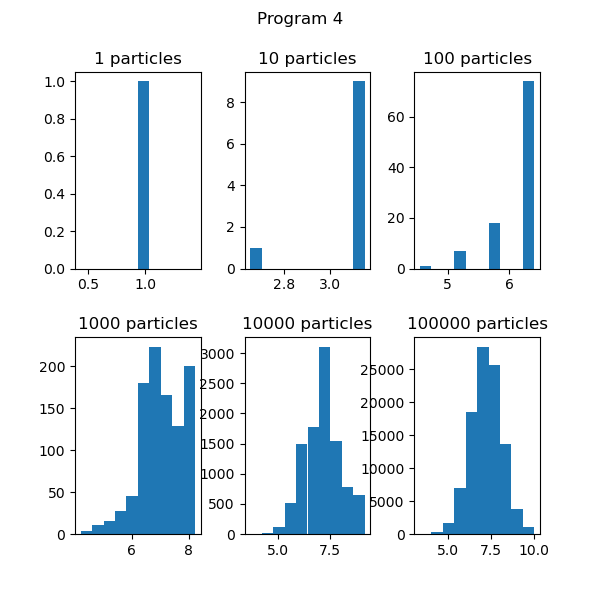
\includegraphics[scale=0.75]{program4_hist}
%	\end{figure}
		

	
	\newpage

	\begin{figure}[h]
	
	\end{figure}
	
	
	\newpage
	
	\section{Snippets of code}
	
	In SMC.py, I filled in resample-particles.
	
		\begin{lstlisting}[language=Python]
		def resample_particles(particles, log_weights):
		    inds = []
		
		    d = dist.Categorical(logits=torch.tensor(log_weights))
		    
		    for i in range(len(particles)):
		        inds.append(d.sample())
		
		    new_particles = [ particles[i] for i in inds ]
		
		    new_weights = torch.logsumexp(torch.tensor(log_weights),0)
		
		    logL = torch.log(torch.tensor(len(log_weights), dtype=float))
		
		    logZ = new_weights - logL
		
		    return logZ, new_particles
		\end{lstlisting}
		
		I modified SMC to get the particles and weights, and check the addresses are all the same.
		
		
		\begin{lstlisting}[language=Python]
		if 'done' in res[2]: #this checks if the calculation is done
		                particles[i] = res[0]
		                if i == 0: 
		                    done = True  # and enforces everything to be the same as the first particle
		                    address = ''
		                else:
		                    if not done:
		                        raise RuntimeError('Failed SMC, finished one calculation before the other')
		            else:
		                address = res[2]['alpha']
		                particles[i]=res
		                weights[i]= res[2]['logW']
		                assert address == particles[0][2]['alpha']
		\end{lstlisting}
			
		Inside evaluator.py I modified sigma for the `observe' case.
		
		\begin{lstlisting}[language=Python]
elif op == 'observe':
            alpha = evaluate(args[0], env=env)
            d = evaluate(args[1], env=env)
            c = evaluate(args[2], env=env)
            k = evaluate(args[3], env=env)

            sigma = {
                'type' : 'observe',
                'logW':d.log_prob(c),
                'alpha': alpha
                     #TODO: put any other stuff you need here
                     }
		\end{lstlisting}
		
		
		
		
	
	
	
	
%	\bibliography{research.bib}
%	\bibliographystyle{plain}
	
	
\end{document}